\section{Simulations and Measurements of the MKI with 19 Screen Conductors}

As can be seen from Fig.~\ref{fig:mki-ip8-heating-2011}, MKI8d had experienced significantly higher temperatures than the other kicker magnets during operation. Although estimated to experience the same degree of power loss within the structure as the other kicker magnets (due to the similarity of the beam screen layout) the large variation in the emissivity of the internal surface of the vacuum tank can have contributed to the higher temperatures observed. As a result of this, and the necessity to find a solution to the high temperatures of the MKIs, which were acting as a severe limiter on the integrated luminousity delivered by the LHC, it was decided to implement an improved beam screen in a replacement magnet in an effort to reduce the power loss in this magnet, and at the same time test some of the principles of future alternative beam screen designs.

The following design features were implemented in the replacement MKI8d (explanations are given with the description, see Fig.~\ref{fig:mki8d-points}):

\begin{enumerate}
\item{19 screen conductors are placed within the beam screen in order to improve the shielding of the ferrite from the beam. These are clustered together, with the 5 empty screen conductor slots closest to the HV busbar to minimise the induced voltage on the screen conductors. Both impedance and electrical simulations have indicated that this will drastically reduce the beam coupling impedance of the MKI, and that the PFN may fire at the operational voltage without inducing electrical breakdowns in the beam screen.}
\item{Elongated metal spheres are placed on the capacitively coupled end of the kicker magnet. These are intended to reduce the field amplification due to any sharp edges at the ends of the screen conductors, thus reducing the possibility of electrical breakdown. This method has some drawbacks due to the need to expand the slots housing the screen conductors to accept the larger elongated spheres.}
\item{The screen conductors are arranged to alternate in length (i.e. there are two lengths of screen conductor in the beam screen) to further reduce the induced potential on the screen conductors. The effect here is for the longer length screen conductors to effectively shield the shorter screen conductors, thus reducing the potential difference between neighbouring screen conductors.}
\end{enumerate}

\begin{figure}
\begin{center}
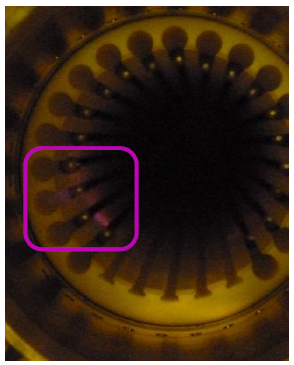
\includegraphics[width=0.5\textwidth]{LHC_MKI/figures/mki8d-balls.png}
\end{center}
\label{fig:mki8d-points}
\caption{The additional screen conductors and the elongated spheres place in MKI8d to reduce both beam coupling impedance and the electric potential build up.}
\end{figure}

Due to the primary motivation for altering the beam screen being the increasing beam-induced heating seen in the kicker magnets the impedance studies were primarily motivated by reducing the real component of the longitudinal beam coupling impedance. Simulations carried out prior to the construction of the magnet predicted that the beam-coupling impedance would be strongly reduced by the inclusion of 4 additional screen conductors. Measurements taken of the magnet  confirmed these simulations to very good accuracy, and shown in Fig.~\ref{fig:mki-19-impedance} along with the measurements and simulations for an MKI with 15 screen conductors. It can be seen that the real component of the beam coupling impedance is reduced drastically across the entire frequency range of concern, and the predicted power loss as a result of the simulated impedance (shown in Tab.~\ref{tab:heating-15-19-cond}) shows that the expected power loss in reduced by a factor of 2-3. Calculations of the thermal evolution of the proposed MKI8d replacement also indicated that the maximum temperature reached would decrease significantly due to this reduced power load[cite]. 

\begin{figure}
\begin{center}
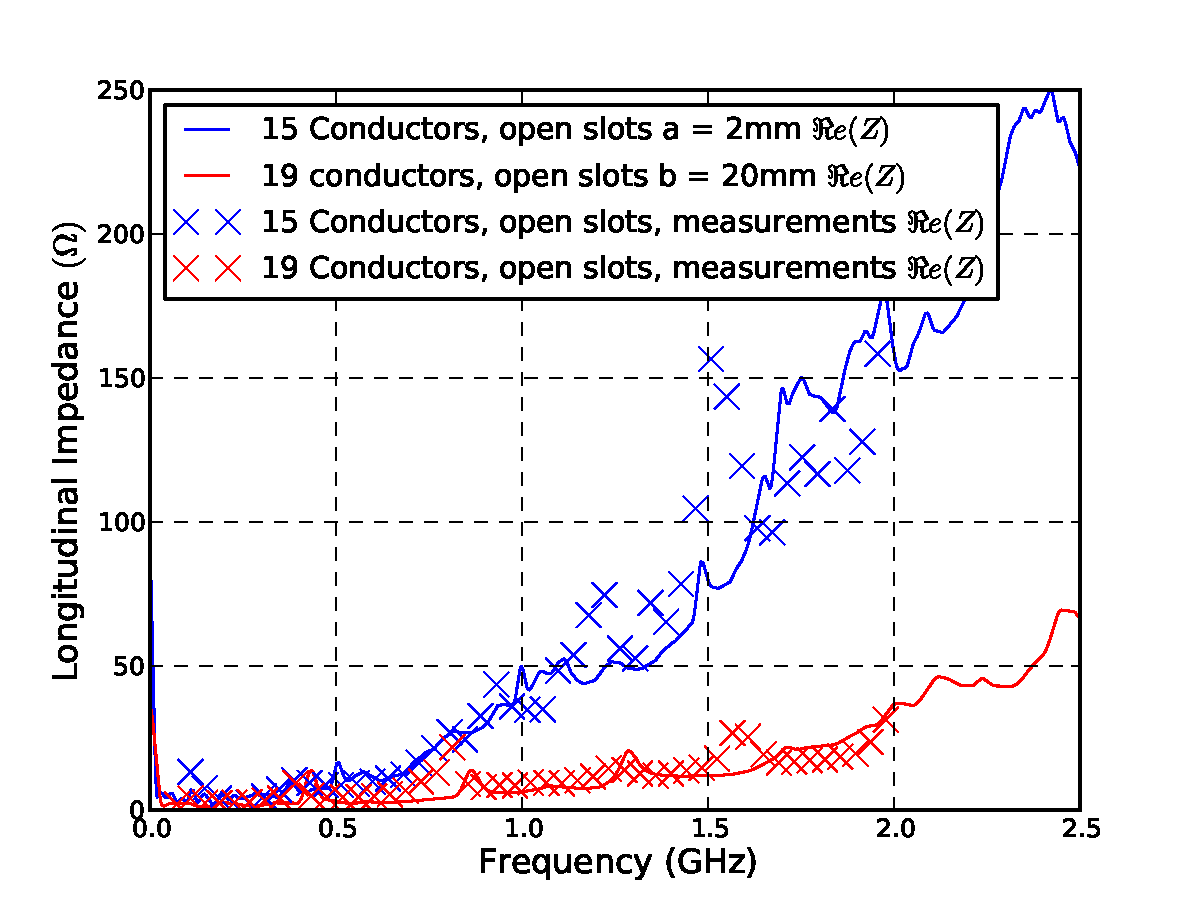
\includegraphics[width=0.8\textwidth]{LHC_MKI/figures/15_19_sims_measured_comparison.pdf}
\end{center}
\label{fig:mki-19-impedance}
\caption{The real component of the longitudinal beam coupling impedance of the reaplcement MKI8d with 19 screen conductors from both simulations and measurements. The corresponding impedance for an MKI with 15 screen conductors is shown for comparison.}
\end{figure}

\begin{table}
\label{tab:heating-15-19-cond}
\caption{The power loss due to the impedance calculated for the MKI with 15 (most common configuration) and 19 (as for MKI8d) screen conductors. Estimates are given assuming a beam with 1380 bunches, seperated by 50ns, with each bunch containing $1.7 \times 10^{11}$ particles. Estimates of the power loss assuming a gaussian, a parabolic and a cos$^{2}$ longitudinal bunch profile are calculated, and a range given for the lowest (typically the gaussian distribution) and highest (typically the cos$^{2}$ distribution due to the large high frequency lobes) values calculated.}
\begin{center}
\begin{tabular}{c | c | c}
Bunch Length (ns) & $P_{loss}$ 15 Screen Conductors & $P_{loss}$ 19 Screen Conductors \\ \hline
1.0 &  134-210 & 50-66 \\ \hline
1.1 &  113-171 & 44-58 \\ \hline
1.2 &  98-143 & 41-52 \\ \hline
1.3 &  86-123 & 40-47 \\ \hline
1.4 &  79-108 & 36-43 \\ \hline
\end{tabular}
\end{center}
\end{table}

\subsection{Temperature of MKI8d after Technical Stop 3}

Due to the promising results of the impedance, electrical and thermal simulations of the proposed MKI8d replacement with 19 screen conductors it was decided to construct the replacement magnet and install it during technical stop 3 (TS3)[cite]. It is said the proof is in the pudding, and in this case mine is exceptionally tasty; Fig.~\ref{fig:heating-mki8-post-ts3} shows the temperatures for the kicker magnets at IP8 both before and after TS3. It can clearly be seen that MKI8d (solid red trace) changes from being the warmest magnet in IP8 - An excellent confirmation of the understanding of the sources of power loss within the kicker magnet and the thermal evolution due to the power loss. From these very promising results a great deal of confidence in the simulation tools for predicting the beam coupling impedance and the understanding of the causes of the beam coupling impedance were acquired. As such more significant changes to the MKI design

\begin{figure}
\begin{center}
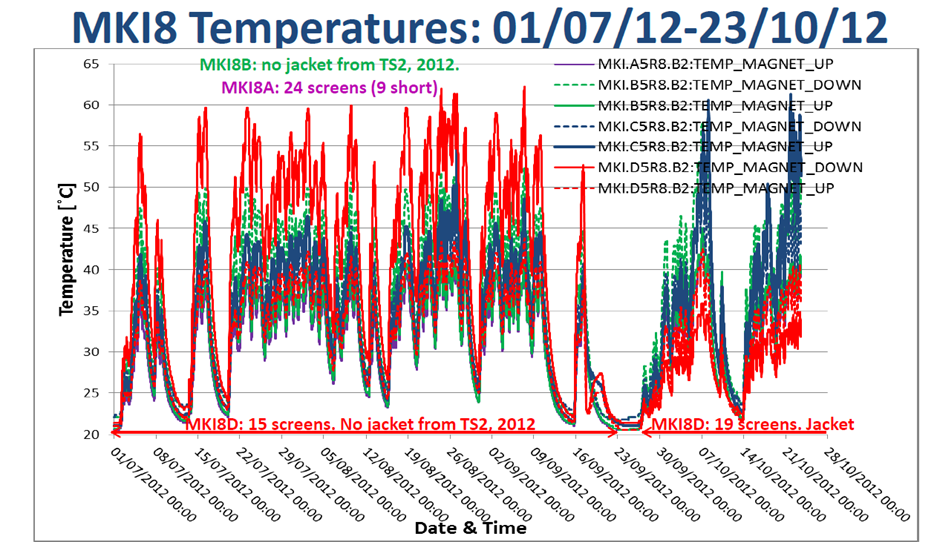
\includegraphics[width=0.6\textwidth]{LHC_MKI/figures/mki8-temps-post-ts3.png}
\end{center}
\label{fig:heating-mki8-post-ts3}
\caption{The temperature profile of the IP8 injection kicker magnets during the time period before and after technical stop 3  (TS3), when the MKI8d was changed from a kicker magnet with 15 screen conductors to one with 19 screen conductors. It can be seen this magnet (solid red trace) goes from being the hottest magnet to the coolest after TS3.}
\end{figure}